\section{Results}
\label{sec:results}

\begin{figure*}[t]
\centering
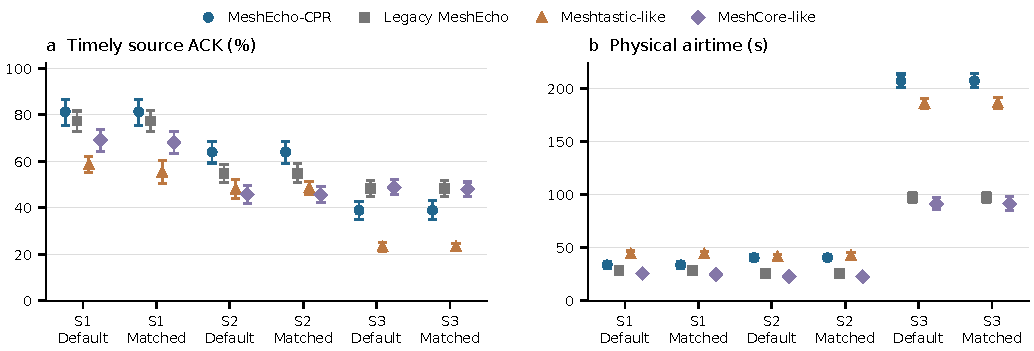
\includegraphics[width=\textwidth]{figures/formal-v2/main_results.pdf}
\caption{Complete main comparison. Points are equal-weight means of 20
seeds; bars are descriptive, unadjusted 95\% bootstrap intervals. Timely
ACK uses all scheduled flows; physical airtime includes all started frames.
The default and matched regimes are distinct cases, not 40 independent seeds.}
\label{fig:main-results}
\end{figure*}

\subsection{The trade-off changes with the operating condition}

Figure~\ref{fig:main-results} retains all four models and both regimes.
CPR's mean timely confirmation falls from 81.30\% in S1 to 63.96\% in S2
and 38.94\% in S3, while mean physical airtime increases from 33.79 to
40.55 and 207.07~s. Its resolved default and matched policies coincide.
The following paired contrasts use the matched regime; changes are
percentage points (pp), and bracketed bounds are descriptive 95\% intervals.

In S1, CPR exceeds legacy MeshEcho by 3.99~pp [$-1.61$, 9.08], with
an airtime ratio of 1.16 [1.06, 1.27]. This does not demonstrate a clear
confirmation improvement over legacy MeshEcho. Relative to Meshtastic-like,
CPR gains 25.99~pp [18.51, 33.31] at a ratio of 0.75 [0.70, 0.81]; relative
to MeshCore-like it gains 13.27~pp [8.04, 18.43] at 1.33 [1.20, 1.47].
These model comparisons include differing discovery and retry semantics.

In S2, CPR gains 9.28~pp [4.42, 14.00] over legacy MeshEcho, at a ratio
of 1.60 [1.50, 1.72]. Against Meshtastic-like the gain is 15.49~pp
[10.26, 20.74], with a ratio of 0.95 [0.91, 0.99]; against MeshCore-like
it is 18.41~pp [14.50, 22.33], with a ratio of 1.81 [1.69, 1.95]. Thus
improved confirmation need not mean reduced airtime.

The S3 result is adverse relative to both route-based comparators.
CPR loses 9.26~pp [$-14.13$, $-4.54$] against legacy MeshEcho and
9.04~pp [$-12.62$, $-4.88$] against MeshCore-like, while spending
2.13 [2.05, 2.24] and 2.29 [2.12, 2.46] times their airtime. It still
exceeds Meshtastic-like confirmation by 15.75~pp [12.25, 19.51], but at
an airtime ratio of 1.11 [1.09, 1.13]. Default-regime results preserve
these directions of the point estimates; parameter matching does not
remove the contention penalty.

\begin{table}[t]
\caption{Timely destination delivery (\%), matched regime. Equal-weight
20-seed means with descriptive 95\% intervals.}
\label{tab:delivery}
\centering\small
\setlength{\tabcolsep}{3pt}
\begin{tabular}{@{}lccc@{}}
\toprule
Model & S1 & S2 & S3 \\
\midrule
MeshEcho-CPR & 95.0 & 78.5 & 67.8 \\
 & [92.1, 97.1] & [75.7, 81.2] & [65.3, 70.2] \\
Legacy MeshEcho & 80.1 & 56.8 & 53.3 \\
 & [76.0, 84.1] & [52.6, 61.1] & [50.3, 56.3] \\
Meshtastic-like & 89.1 & 75.6 & 61.4 \\
 & [85.8, 92.0] & [72.4, 78.8] & [60.0, 62.7] \\
MeshCore-like & 72.8 & 48.7 & 53.4 \\
 & [68.3, 77.4] & [45.3, 52.5] & [50.4, 56.3] \\
\bottomrule
\end{tabular}
\end{table}

Delivery and confirmation diverge (Table~\ref{tab:delivery}). CPR has
67.81\% timely destination delivery in S3 despite only 38.94\%
confirmation. The corresponding legacy MeshEcho values are 53.29\%
and 48.20\%. Extra delivery alone therefore cannot establish the quality
of a confirmed transaction, and the gap does not by itself isolate the
cause of missing ACKs.

\subsection{Recovery helps disrupted paths and hurts under contention}

\begin{figure*}[t]
\centering
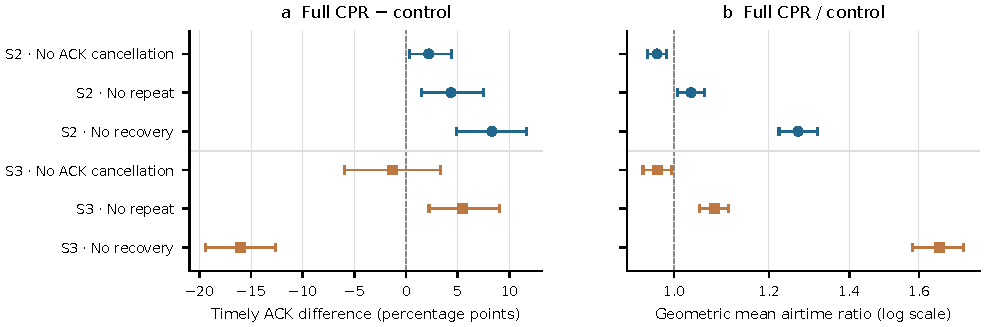
\includegraphics[width=\textwidth]{figures/formal-v2/component_effects.pdf}
\caption{Clean component controls in matched S2/S3, with all 20 paired
seeds. Panel (a) is full CPR minus the named control; panel (b) is the
geometric mean full/control physical-airtime ratio on a log scale.
Intervals are descriptive and unadjusted. Recovery's confirmation effect
reverses between the two settings.}
\label{fig:components}
\end{figure*}

Figure~\ref{fig:components} isolates each declared switch. In S2,
full CPR versus no recovery gains 8.32~pp [4.90, 11.63], at an airtime
ratio of 1.27 [1.22, 1.32]. In S3, the same contrast loses 15.99~pp
[$-19.41$, $-12.64$] and raises airtime to 1.66 [1.58, 1.74] times
that of the control. Removing recovery yields 54.93\% confirmation
and 125.21~s mean airtime, versus 38.94\% and 207.07~s for full CPR.
Its timely delivery is 64.94\%, versus 67.81\% for full CPR. Recovery
can therefore increase destination delivery while substantially harming
source confirmation in this contention setting.

The repeat contrast is positive in both settings: full versus no repeat
gains 4.35~pp [1.48, 7.51] in S2 and 5.43~pp [2.23, 9.01] in S3,
with airtime ratios 1.033 [1.007, 1.060] and 1.081 [1.051, 1.110].
The control preserves the nominal observation slot, so this comparison
includes the effects of removing the physical repeat and its downstream
contention while retaining the defined recovery timing rule.

ACK cancellation reduces paired airtime in S2 and S3: ratios are
0.968 [0.950, 0.986] and 0.968 [0.942, 0.995]. Its confirmation effect
is 2.20~pp [0.36, 4.38] in S2 but $-1.29$~pp [$-5.99$, 3.38] in
S3. The latter interval includes effects in both directions. These are
whole-policy paired costs, not savings inferred by multiplying canceled
copies by a nominal frame duration.

\subsection{Observed exposure and the boundary of mechanism evidence}

The complete S2 CPR population contains 648 scheduled flows per regime.
Among them, 85 routed initial transmissions start inside the fault window
with a carried path crossing a fault edge; each path had an accepted ACK
before the fault on the same generation. All 20 seeds expose this condition.
Of these 85 flows, 82 physically repeat and 78 start recovery; 24 deliver
on time, 18 receive a timely ACK, and 61 do not deliver on time. Every
successful first delivery and timely ACK in this subset is associated
with recovery marker 2. Twenty-three deliveries and 17 ACKs complete
within the active fault along avoiding paths. These stage associations
support mechanism interpretation; the no-recovery contrast supplies the
separate policy-effect evidence.

Across the full S2 population, 159 physical transmissions on fault edges
involve 87 flows: 78 initial DATA, 80 repeat DATA, and one ACK. None of
these intended receptions decodes. This population differs from the 85
initial-path crossings. Four of 25 fault-active flows whose initial send
precedes 80~s make a later actual fault-edge attempt. Exposure is measured
at physical TX start, without excluding cross-boundary failures or
unexposed scheduled flows from the main estimand.

S1 also exercises routed operation: per regime, 480 routed and 168
initial-flood starts serve the 648 flows; its 526 accepted ACKs traverse
four or six hops. S3 has 3059 scheduled flows, 2445 routed and 608
initial-flood starts, 1890 repeats, and 1597 recoveries. Intended-hop
capture-collision and half-duplex counts rise from 227/35 in S1 to
3228/887 in S3. These correlated hop/attempt outcomes indicate increased
contention, not independent flow failures. S3 has six source-state
capacity refusals and 52 protocol-no-start requests. Relay-ledger eviction
and capacity cancellation remain zero; peak ledger occupancy is not
reconstructed, so no measured memory-capacity advantage is claimed.

\subsection{Finite deadline and load response}

\begin{figure*}[t]
\centering
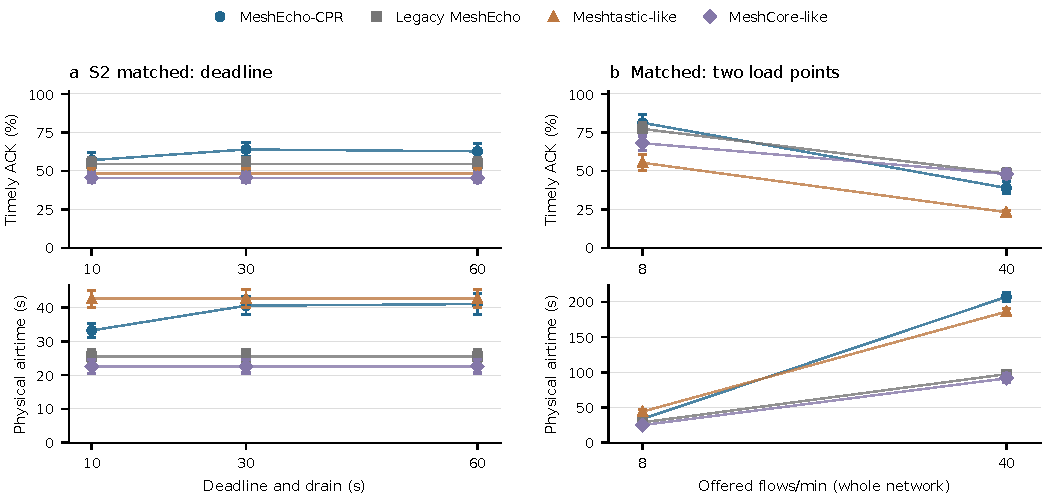
\includegraphics[width=\textwidth]{figures/formal-v2/robustness.pdf}
\caption{Prespecified finite response. (a) The S2 matched deadline axis
also changes drain duration; generation is always 240 s. (b) The two
fault-free offered loads reuse S1/S3 matched. Lines join observed points
only. All estimates use 20 seeds with descriptive 95\% intervals; no
cross-deadline inferential contrast or saturation threshold is claimed.}
\label{fig:robustness}
\end{figure*}

At deadlines of 10, 30, and 60~s, CPR's mean confirmation is 57.01\%,
63.96\%, and 62.74\%, with mean airtime 33.22, 40.55, and 41.05~s
(Fig.~\ref{fig:robustness}). The confirmation intervals are [51.75, 61.85],
[59.15, 68.57], and [57.32, 67.93]\%. There is no monotonic improvement
across all three points. Mean physical repeats per run are 6.3, 9.1, and
11.2; recovery starts are 0, 7.1, and 9.4. The 10-s case records 99
rejections specifically labeled \texttt{recovery-deadline-infeasible}.
Stale-route rejections are counted separately. Comparator point means
are unchanged across these three deadline/drain settings. The two load
points reproduce the S1/S3 reversal and do not locate its onset.

\subsection{Latency and physical-cost context}

\begin{figure*}[t]
\centering
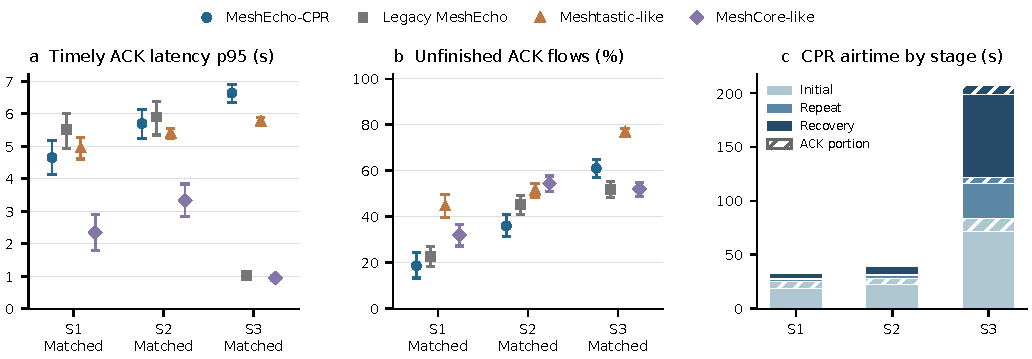
\includegraphics[width=\textwidth]{figures/formal-v2/latency_cost.pdf}
\caption{Matched main cases. (a) Mean of seed-level p95 latency among
timely ACK successes. (b) Unfinished ACK fraction over all scheduled
flows. (c) CPR physical airtime by source stage, including that stage's
relay traffic; hatching marks ACK airtime. Panels (a,b) show descriptive
95\% intervals; the additive cost partition shows means only.}
\label{fig:latency-cost}
\end{figure*}

The mean of CPR's seed-level timely-ACK latency p95 values is 4.65, 5.70,
and 6.63~s for S1/S2/S3 (Fig.~\ref{fig:latency-cost}). Its unfinished
ACK fractions are 18.70\%, 36.04\%, and 61.06\%. The short successful
latencies of the route-based comparators in S3 coexist with more than
half their flows lacking timely confirmation. Success-only latency is
therefore not a complete responsiveness ranking. CPR's mean airtime per
timely destination delivery rises from 1.11 to 1.61 and 2.01~s. The
stage partition reconstructs full physical airtime, including ACKs;
recovery occupies a large part of S3's cost. It neither measures device
energy nor assigns an independent confidence interval to each stacked
component.
